\documentclass[twocolumn]{autart}

%\input{doiCmd}
%\RequirePackage{doi}
\usepackage[
	pdftitle={Hic sunt dracones! the modern unknown Data Dragons},
	pdfsubject={Hic sunt dracones! the modern unknown Data Dragons},
	pdfauthor={Florian Thiery, Martina Trognitz, Ethan Gruber, David Wigg-Wolf},
	pdfkeywords={Linked Data, Linked Open Data, Five Star Data, FAIR Data, Semantic Web, Data Dragon}
]{hyperref}

\usepackage{graphicx}          % Include this line if your 
                               % document contains figures,
%\usepackage[dvips]{epsfig}    % or this line, depending on which
                               % you prefer.
\usepackage{verbatimbox}

\usepackage[german, english]{babel} 

\usepackage{mnsymbol}

\usepackage{url}

\usepackage{xcolor}

\begin{document}\selectlanguage{english}

\begin{frontmatter}
%\runtitle{Insert a suggested running title}  % Running title for regular 
                                              % papers but only if the title  
                                              % is over 5 words. Running title 
                                              % is not shown in output.

\title{Hic sunt dracones! \protect\\ The modern unknown Data Dragons}
                                               

\author[FT]{Florian Thiery},\author[MT]{Martina Trognitz},\author[EG]{Ethan Gruber},\author[DWW]{David Wigg-Wolf}

\address[FT]{ORCID: 0000-0002-3246-3531 \protect\\ R\"omisch-Germanisches Zentralmuseum, Mainz, Germany}                                        

\address[MT]{ORCID: 0000-0003-0485-6861 \protect\\ Austrian Centre for Digital Humanities at Austrian Academy of Sciences, Austria}

\address[EG]{ORCID: 0000-0002-4691-9747 \protect\\ American Numismatic Society, USA}

\address[DWW]{ORCID: 0000-0002-8604-544X \protect\\ R\"omisch-Germanische Kommission des Deutschen Arch\"aologischen Instituts, Germany}

          
\begin{keyword}                             
Linked Data; Linked Open Data; Five Star Data; FAIR Data; Semantic Web; Data Dragon. 
\end{keyword}

\begin{abstract}                         

The world of digital data is full of unknown data, with are not FAIR (Findable, Accessible, Interoperable and Reusable). This modern species of dragons on a (digital) map of the internet as sign for unknown and dangerous areas, the unknown digital data dragons, have to be resolved by digital techniques. We could use the Semantic Web and all of its ideas for this challenge. This paper focuses on data dragons in the humanities domain, especially in archaeology and proposes ideas to overcome the data dragons to achieve FAIR LOUD in archaeology!

\end{abstract}

\end{frontmatter}

\section{Hic sunt dracones digitales!}

In historical maps (cf. Fig.~\ref{map}), the phrase \textbf{Hic sunt dracones} (engl. \textit{here be dragons}) is used to describe areas which were unknown to the map creator \cite{wuttke_here_2019}. 

\begin{figure}[!htb]
\begin{center}
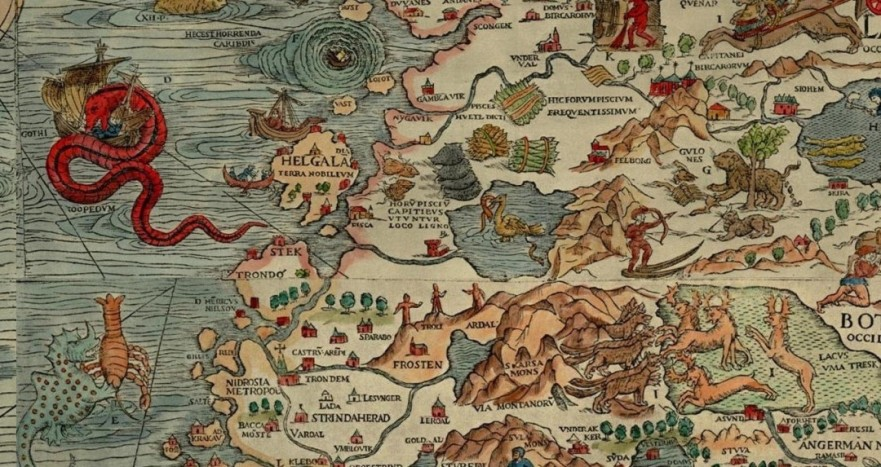
\includegraphics[width=8cm]{Beyond-This-here-be-no-dragons-blog-copy-881x467.jpg}
\caption{Nature and Science, https://t1p.de/wmtz}
\label{map}
\end{center}
\end{figure}

Today the WWW gives researchers the possibility of sharing their research (data) and enables the community to participate in the scientific discourse to create previously unknown knowledge. But much of this shared data are not findable or accessible, thus resulting in modern \textbf{unknown data dragons}. Often these \textbf{data dragons} (cf. Fig.~\ref{datadragon}) lack connections to other datasets, i.e. they are not interoperable and in some cases even lack usefulness or usability. To overcome these shortcomings, a set of techniques, standards and recommendations can be used: \textit{Semantic Web} and \textit{Linked Open Data}, the \textit{FAIR principles} and \textit{LOUD}.

\begin{figure}[!htb]
\begin{center}

\includegraphics[width=6cm]{datadragon.png}
\caption{Data Dragon}
\label{datadragon}
\end{center}
\end{figure}

\section{Shout it out, FAIR and LOUD!}

Tim Berners-Lee introduced the concept of \textit{Semantic Web}, where he suggested using the ideas of Open Data, semantically described resources and links, as well as usable (machine readable) interfaces and applications for creating a \textit{Giant Global Graph}. In 2016 the FAIR principles were introduced \cite{wilkinson_fair_2016}: Research data and its metadata have to be \textbf{F}indable, \textbf{A}ccessible, \textbf{I}nteroperable and \textbf{R}eusable. Linked Data (cf. Fig.~\ref{ld}) is an essential part of the FAIR principles: \frqq The Semantic Web isn't just about putting data on the web. It is about making links, so that a person or machine can explore the web of data\flqq\cite{berners-lee_linked_2006}. Publishing research data as HTTP URIs with RDF content containing links to other resources makes data FAIR! 

\begin{figure}[!htb]
\begin{center}
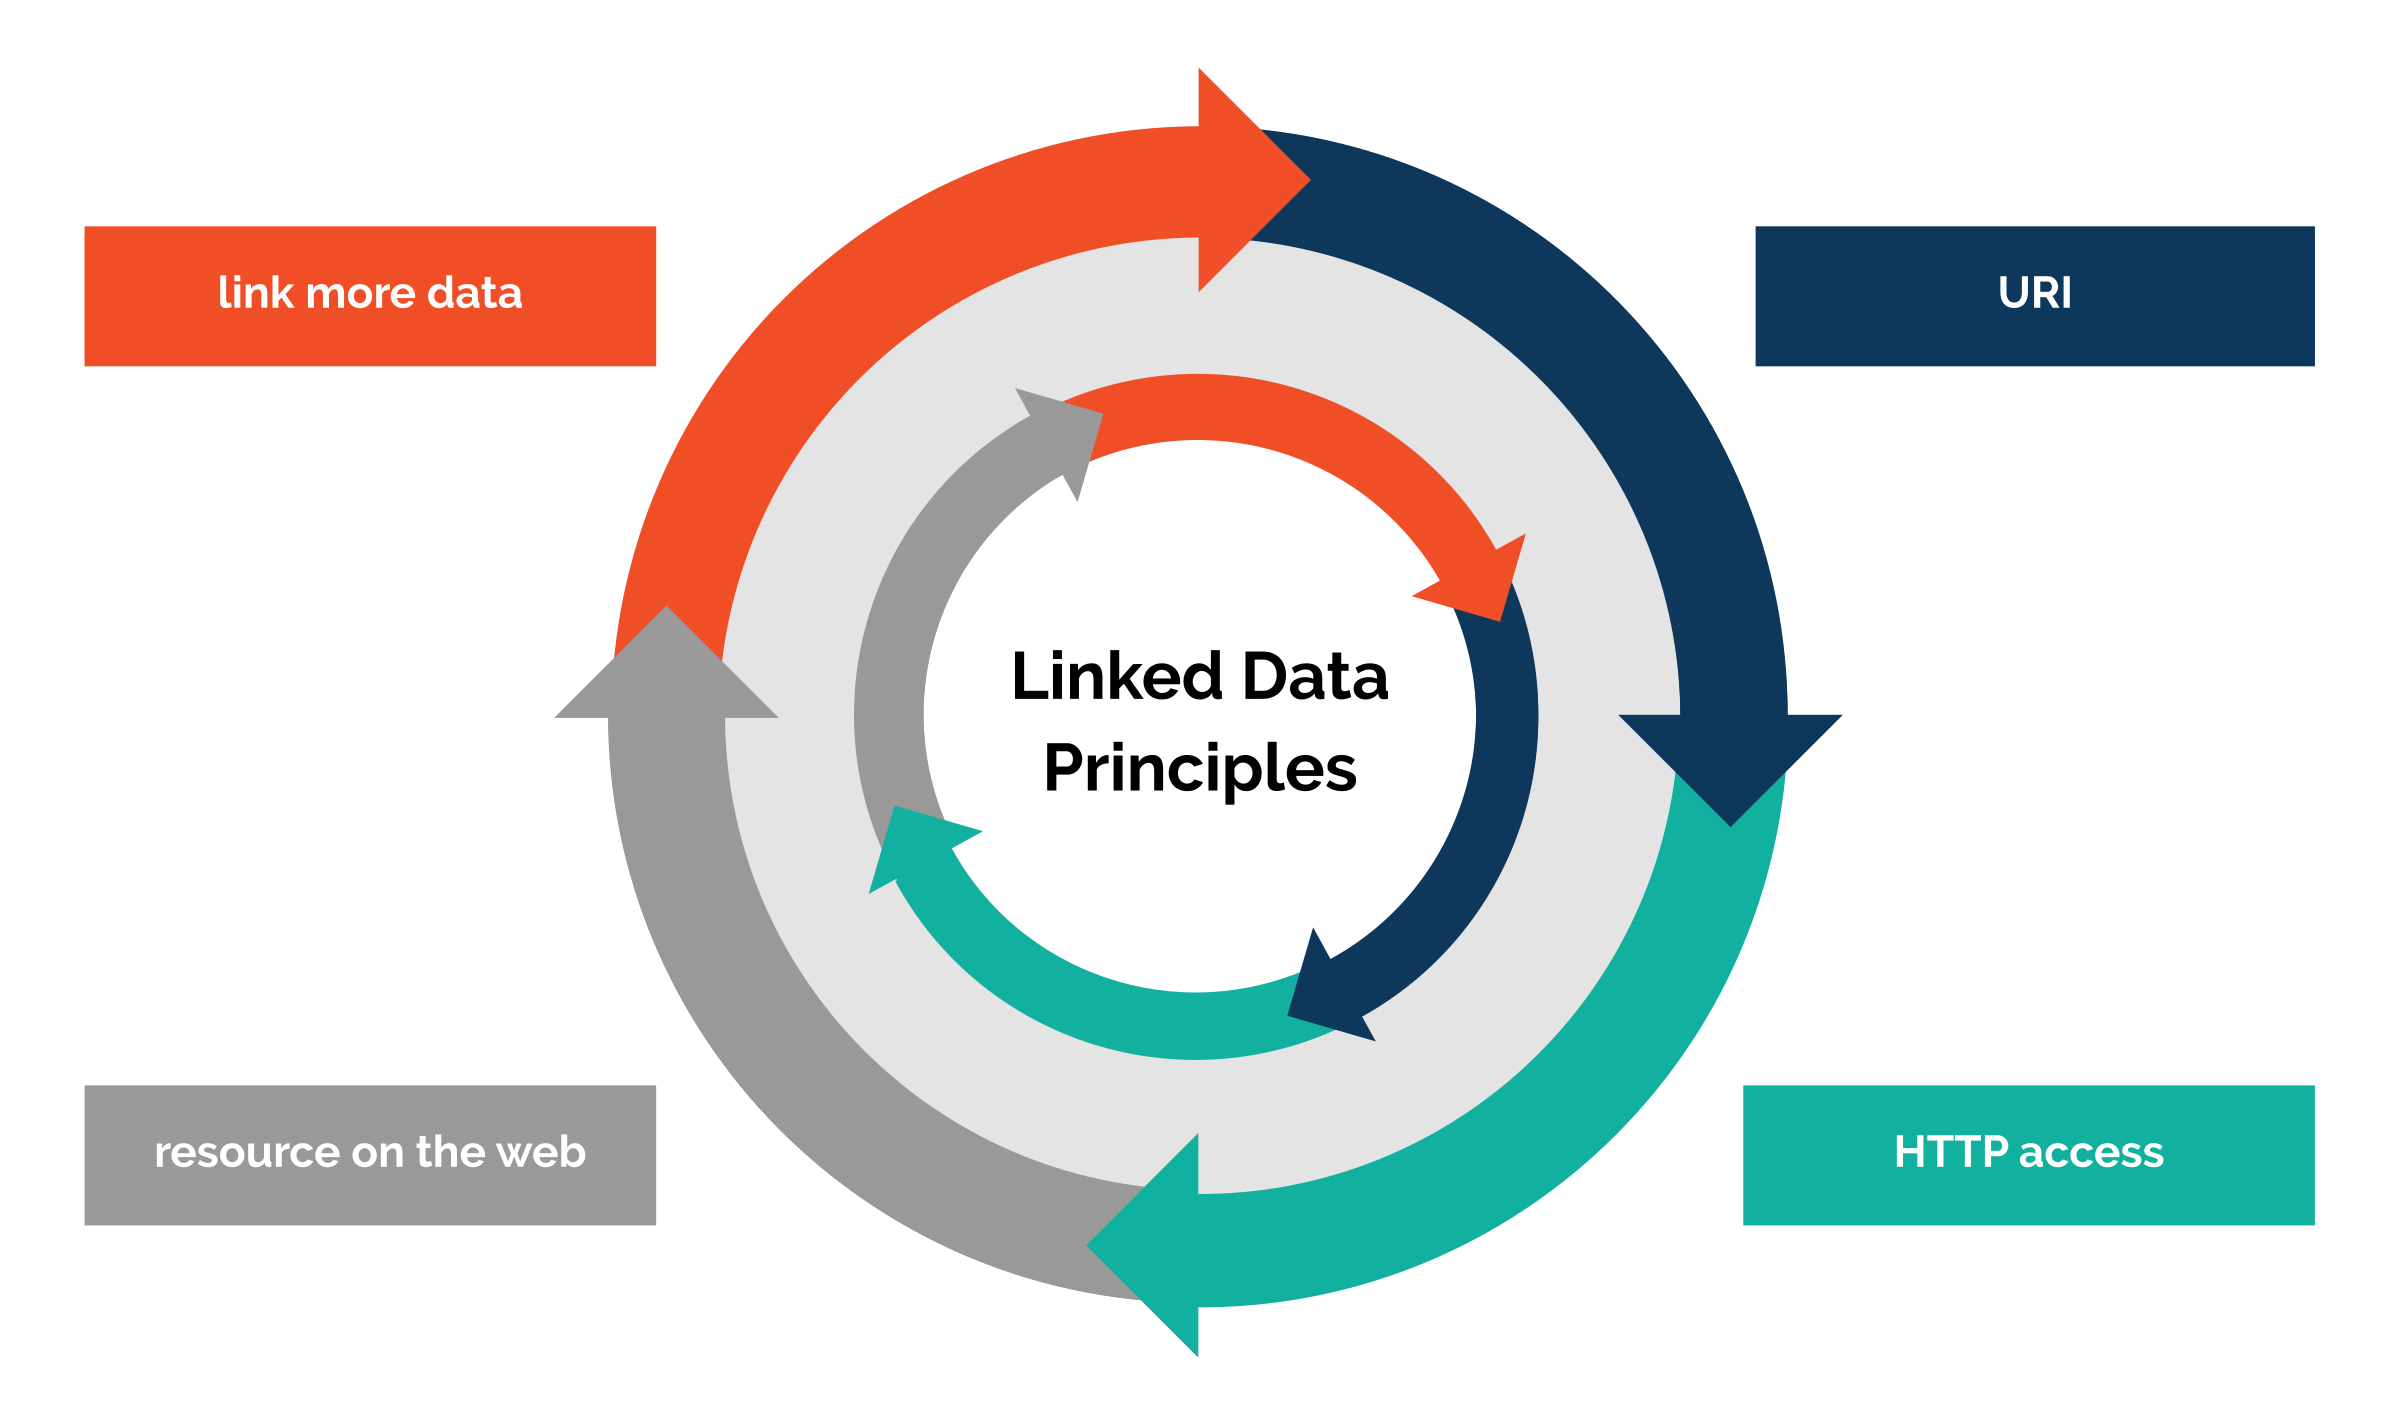
\includegraphics[width=8cm]{Linked_Data_Principles.png}
\caption{Linked Data, Florian Thiery [CC BY 4.0]}
\label{ld}
\end{center}
\end{figure}

On top of that, these data should be \textit{open} for access, re-use and universal participation \cite{open_data_handbook_what_2019}. A five star rating system of openness \cite{hausenblas_5_star_2012} was introduced to rate Linked Data, i. e. \frqq Linked Open Data (LOD, cf. Fig.~\ref{5sd}) is Linked Data which is released under an open licence\flqq\cite{berners-lee_linked_2006}. Furthermore, LOD have to be `usable` for scientists and programmers to take advantage of all the LOD power. Following the LOUD (cf. Fig.~\ref{loud}) principles\cite{sanderson_loud_2019} will make LOD even more FAIR.

\begin{figure}[!htb]
\begin{center}
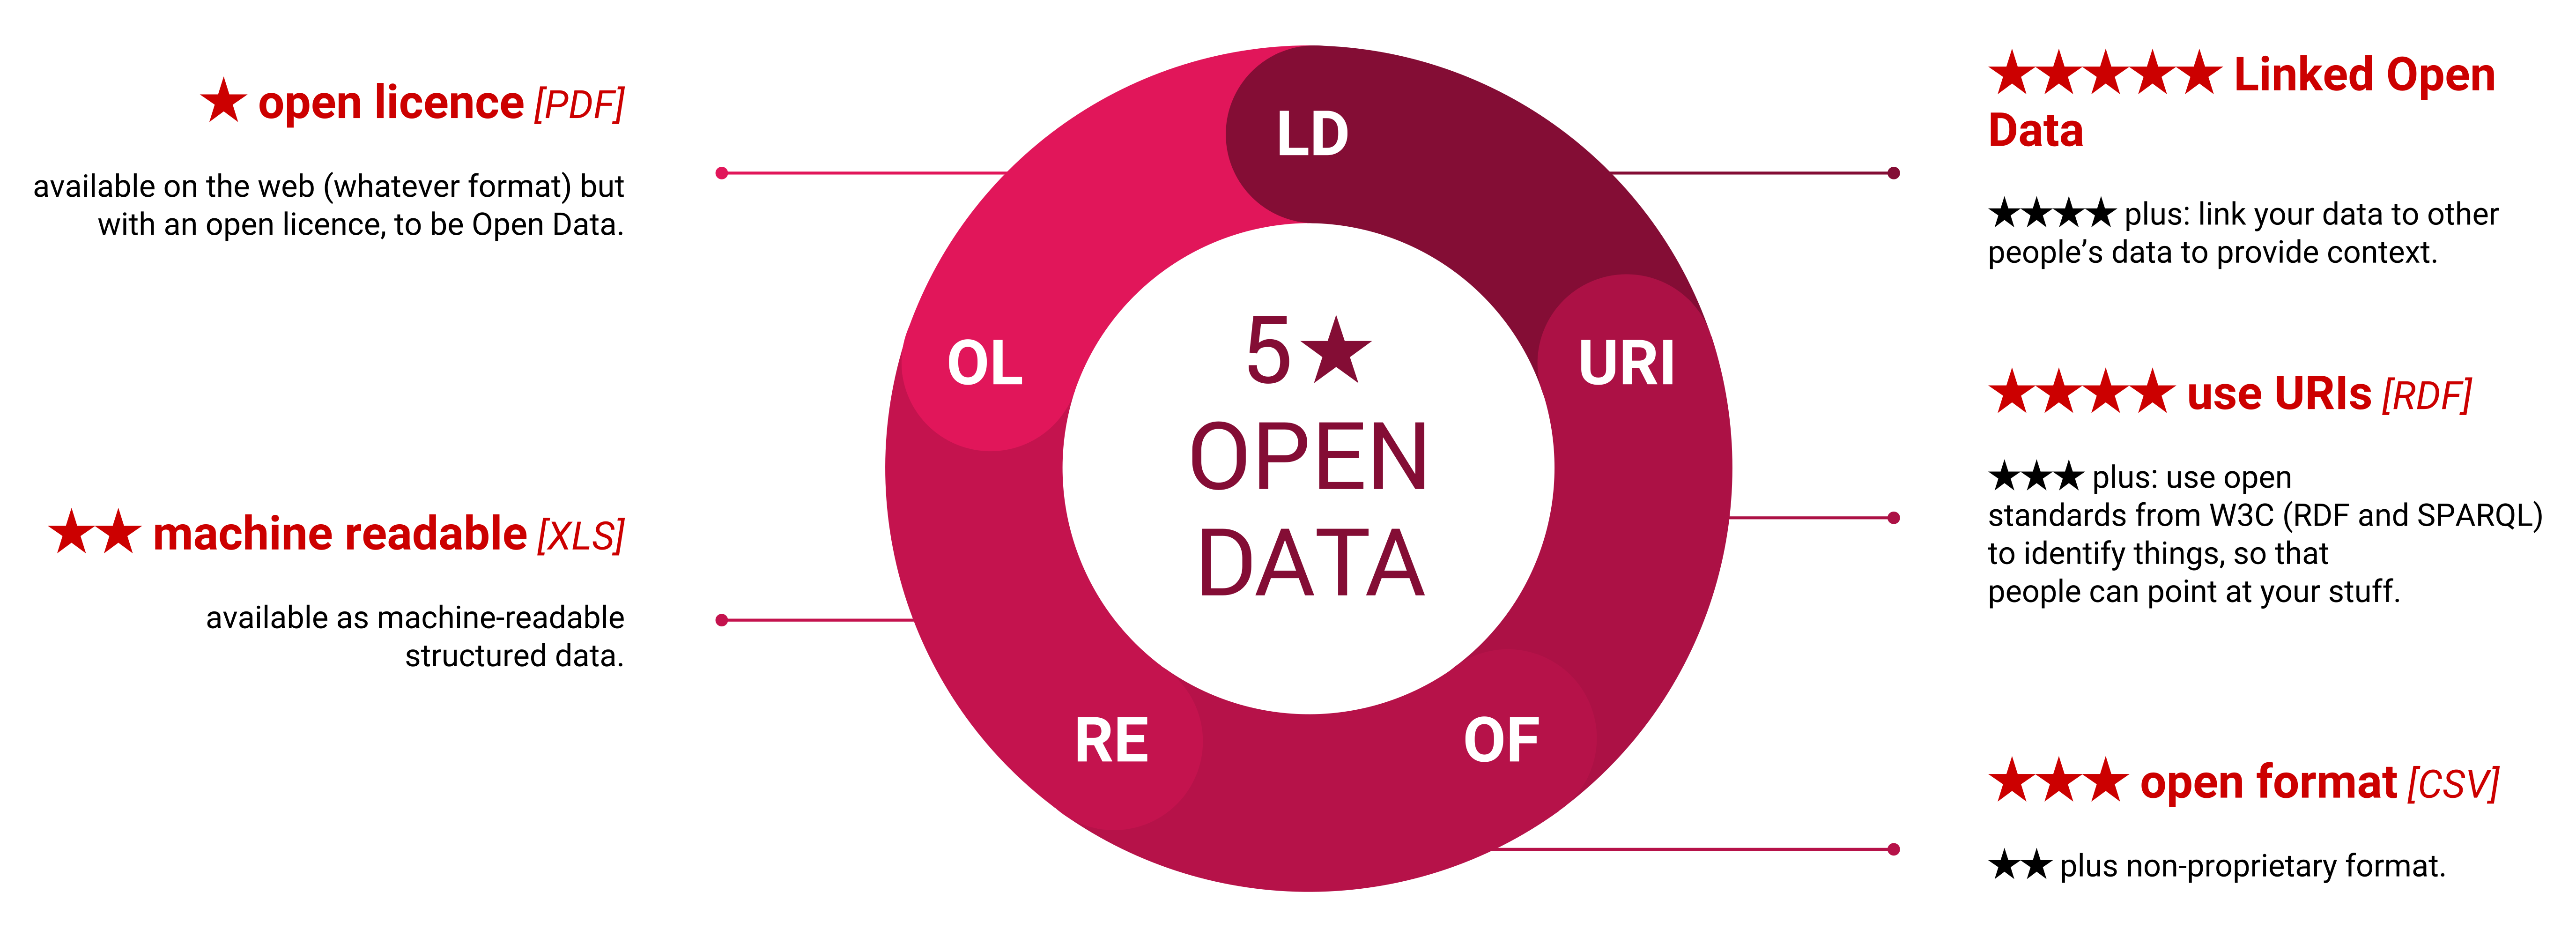
\includegraphics[width=8cm]{5_Star_Open_Data.png}
\caption{5 Star Open Data, Florian Thiery [CC BY 4.0]}
\label{5sd}
\end{center}
\end{figure}

\begin{figure}[!htb]
\begin{center}
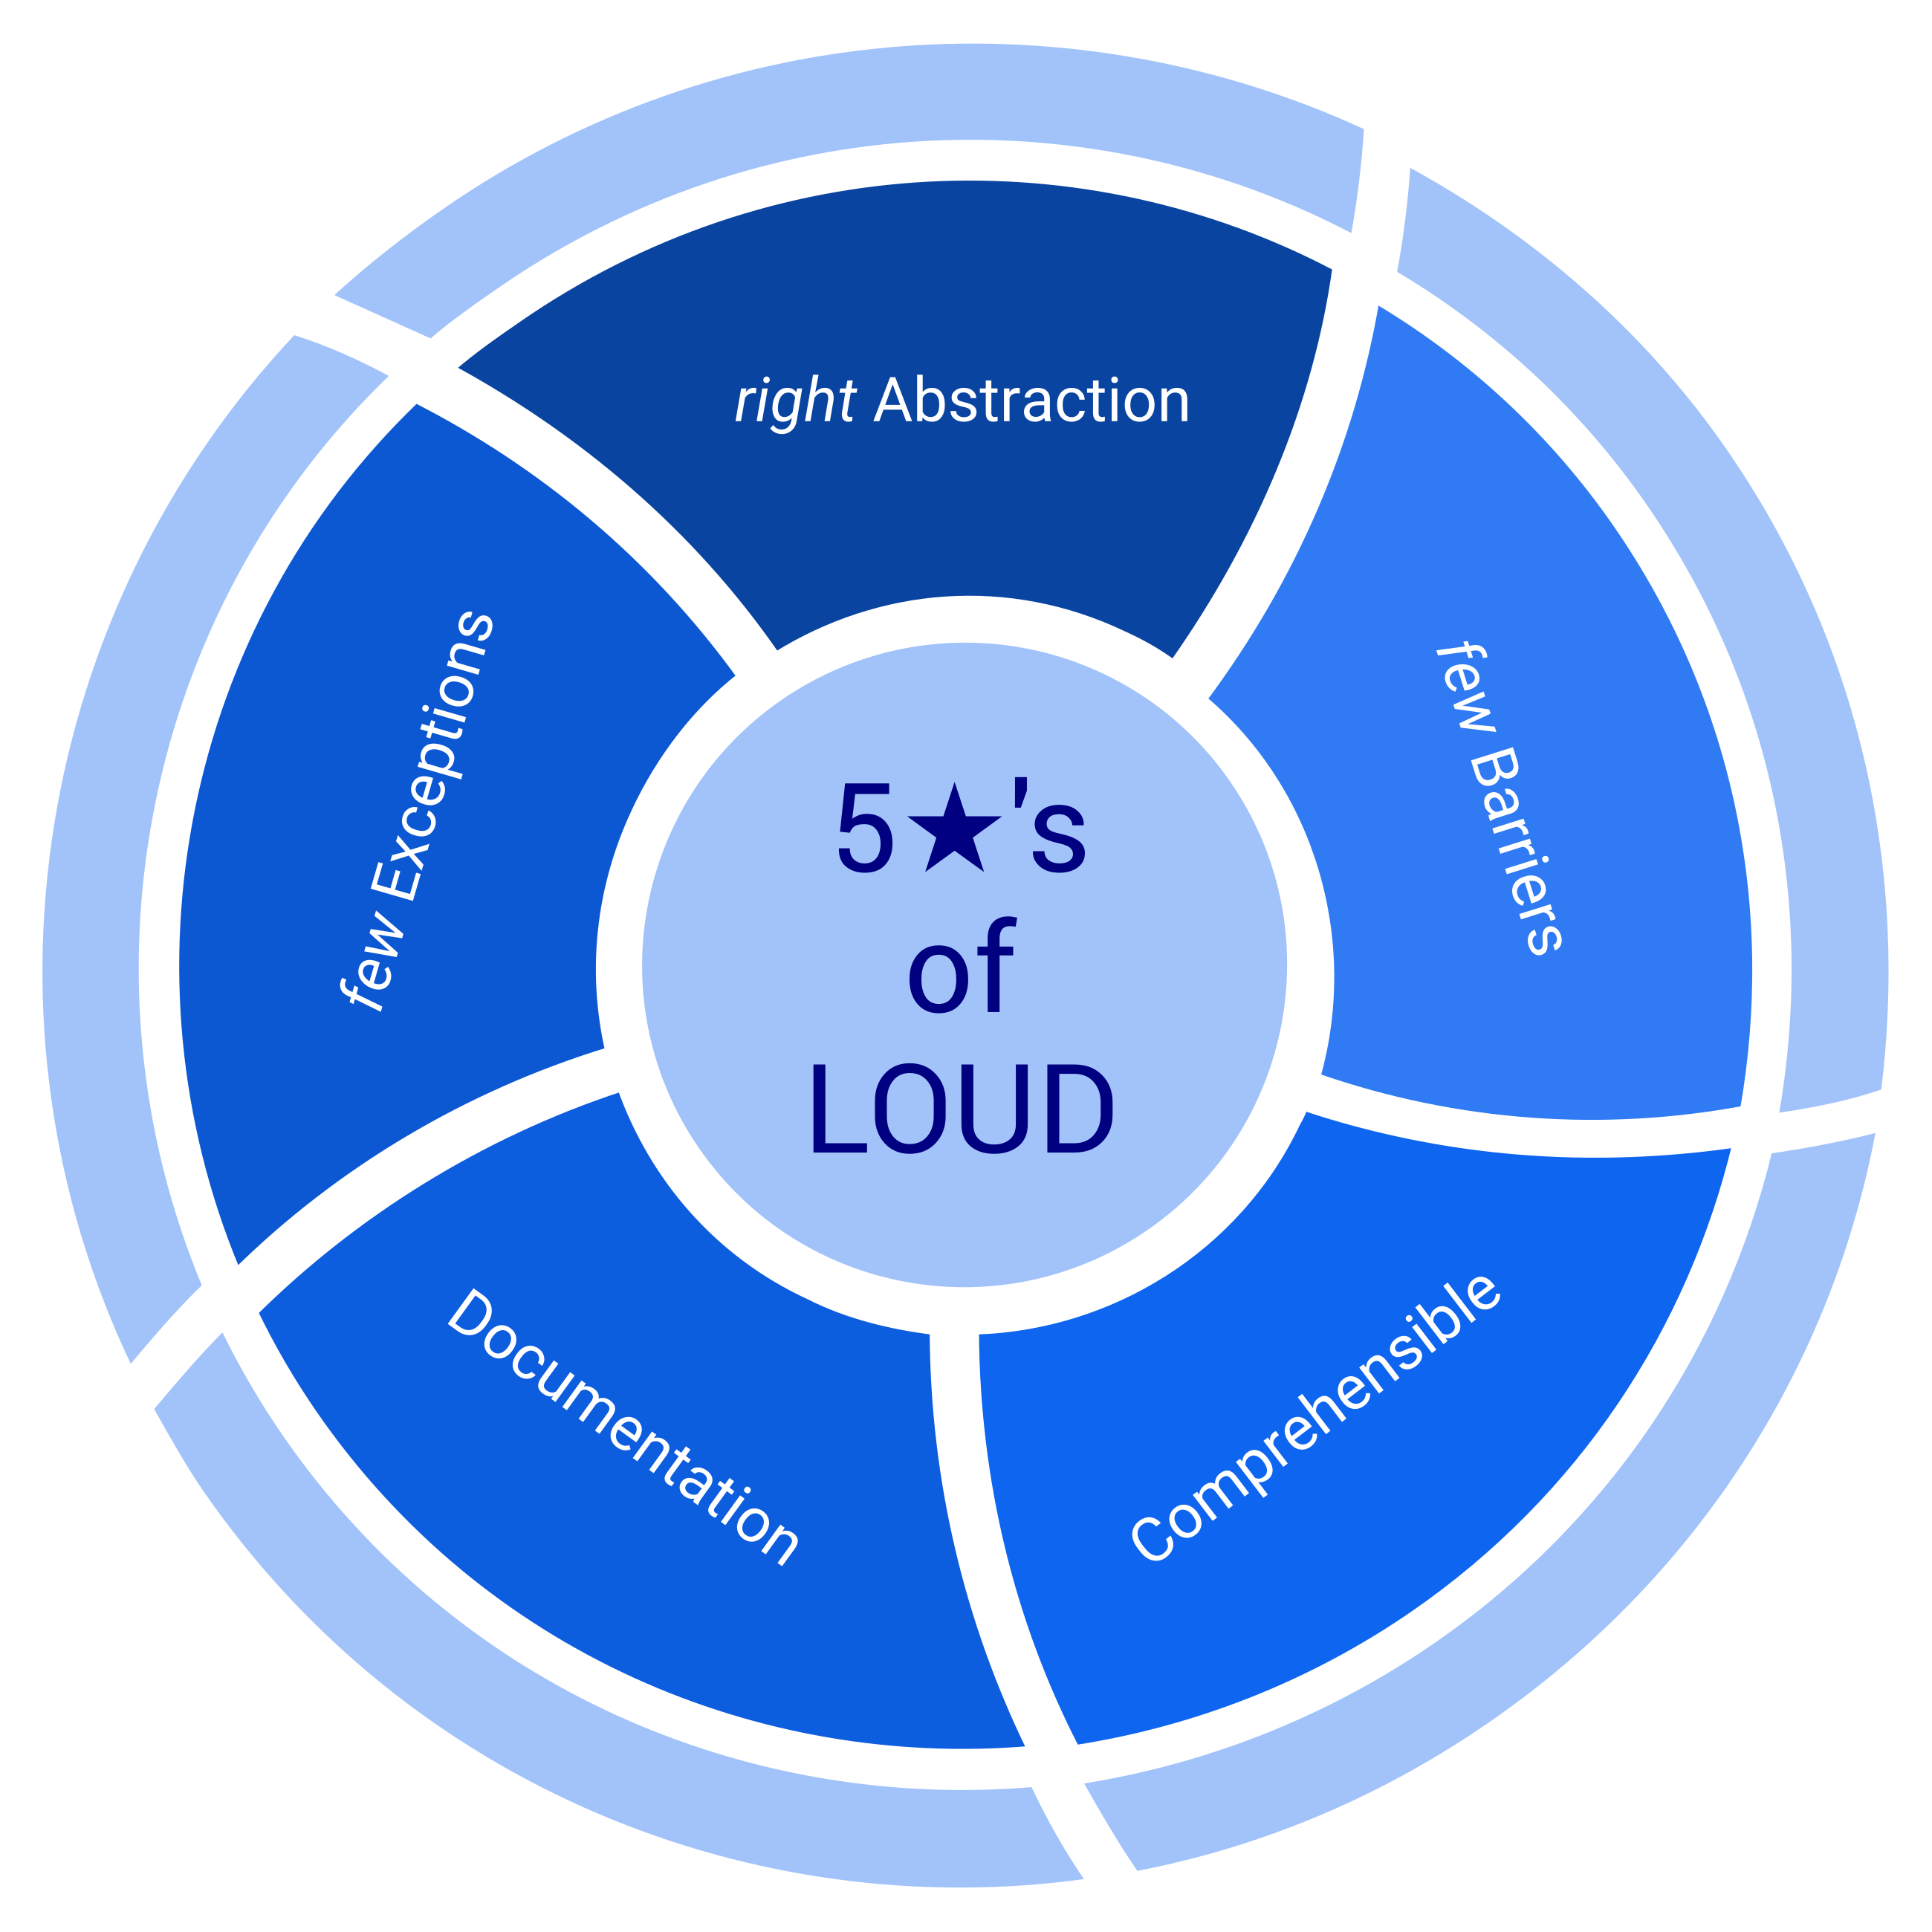
\includegraphics[width=8cm]{5_Star_LOUD.png}
\caption{5 Star LOD, Florian Thiery [CC BY 4.0]}
\label{loud}
\end{center}
\end{figure}

Merging all these principles to create FAIR and LOUD research data results in the \textit{Sphere 7 Data Model} (cf. Fig.~\ref{ssd}) \cite{thiery_sphere_2019}, which enables a wide array of digital humanities and archaeological (web-)applications using LOUD and FAIR data.

\begin{figure}[!htb]
\begin{center}
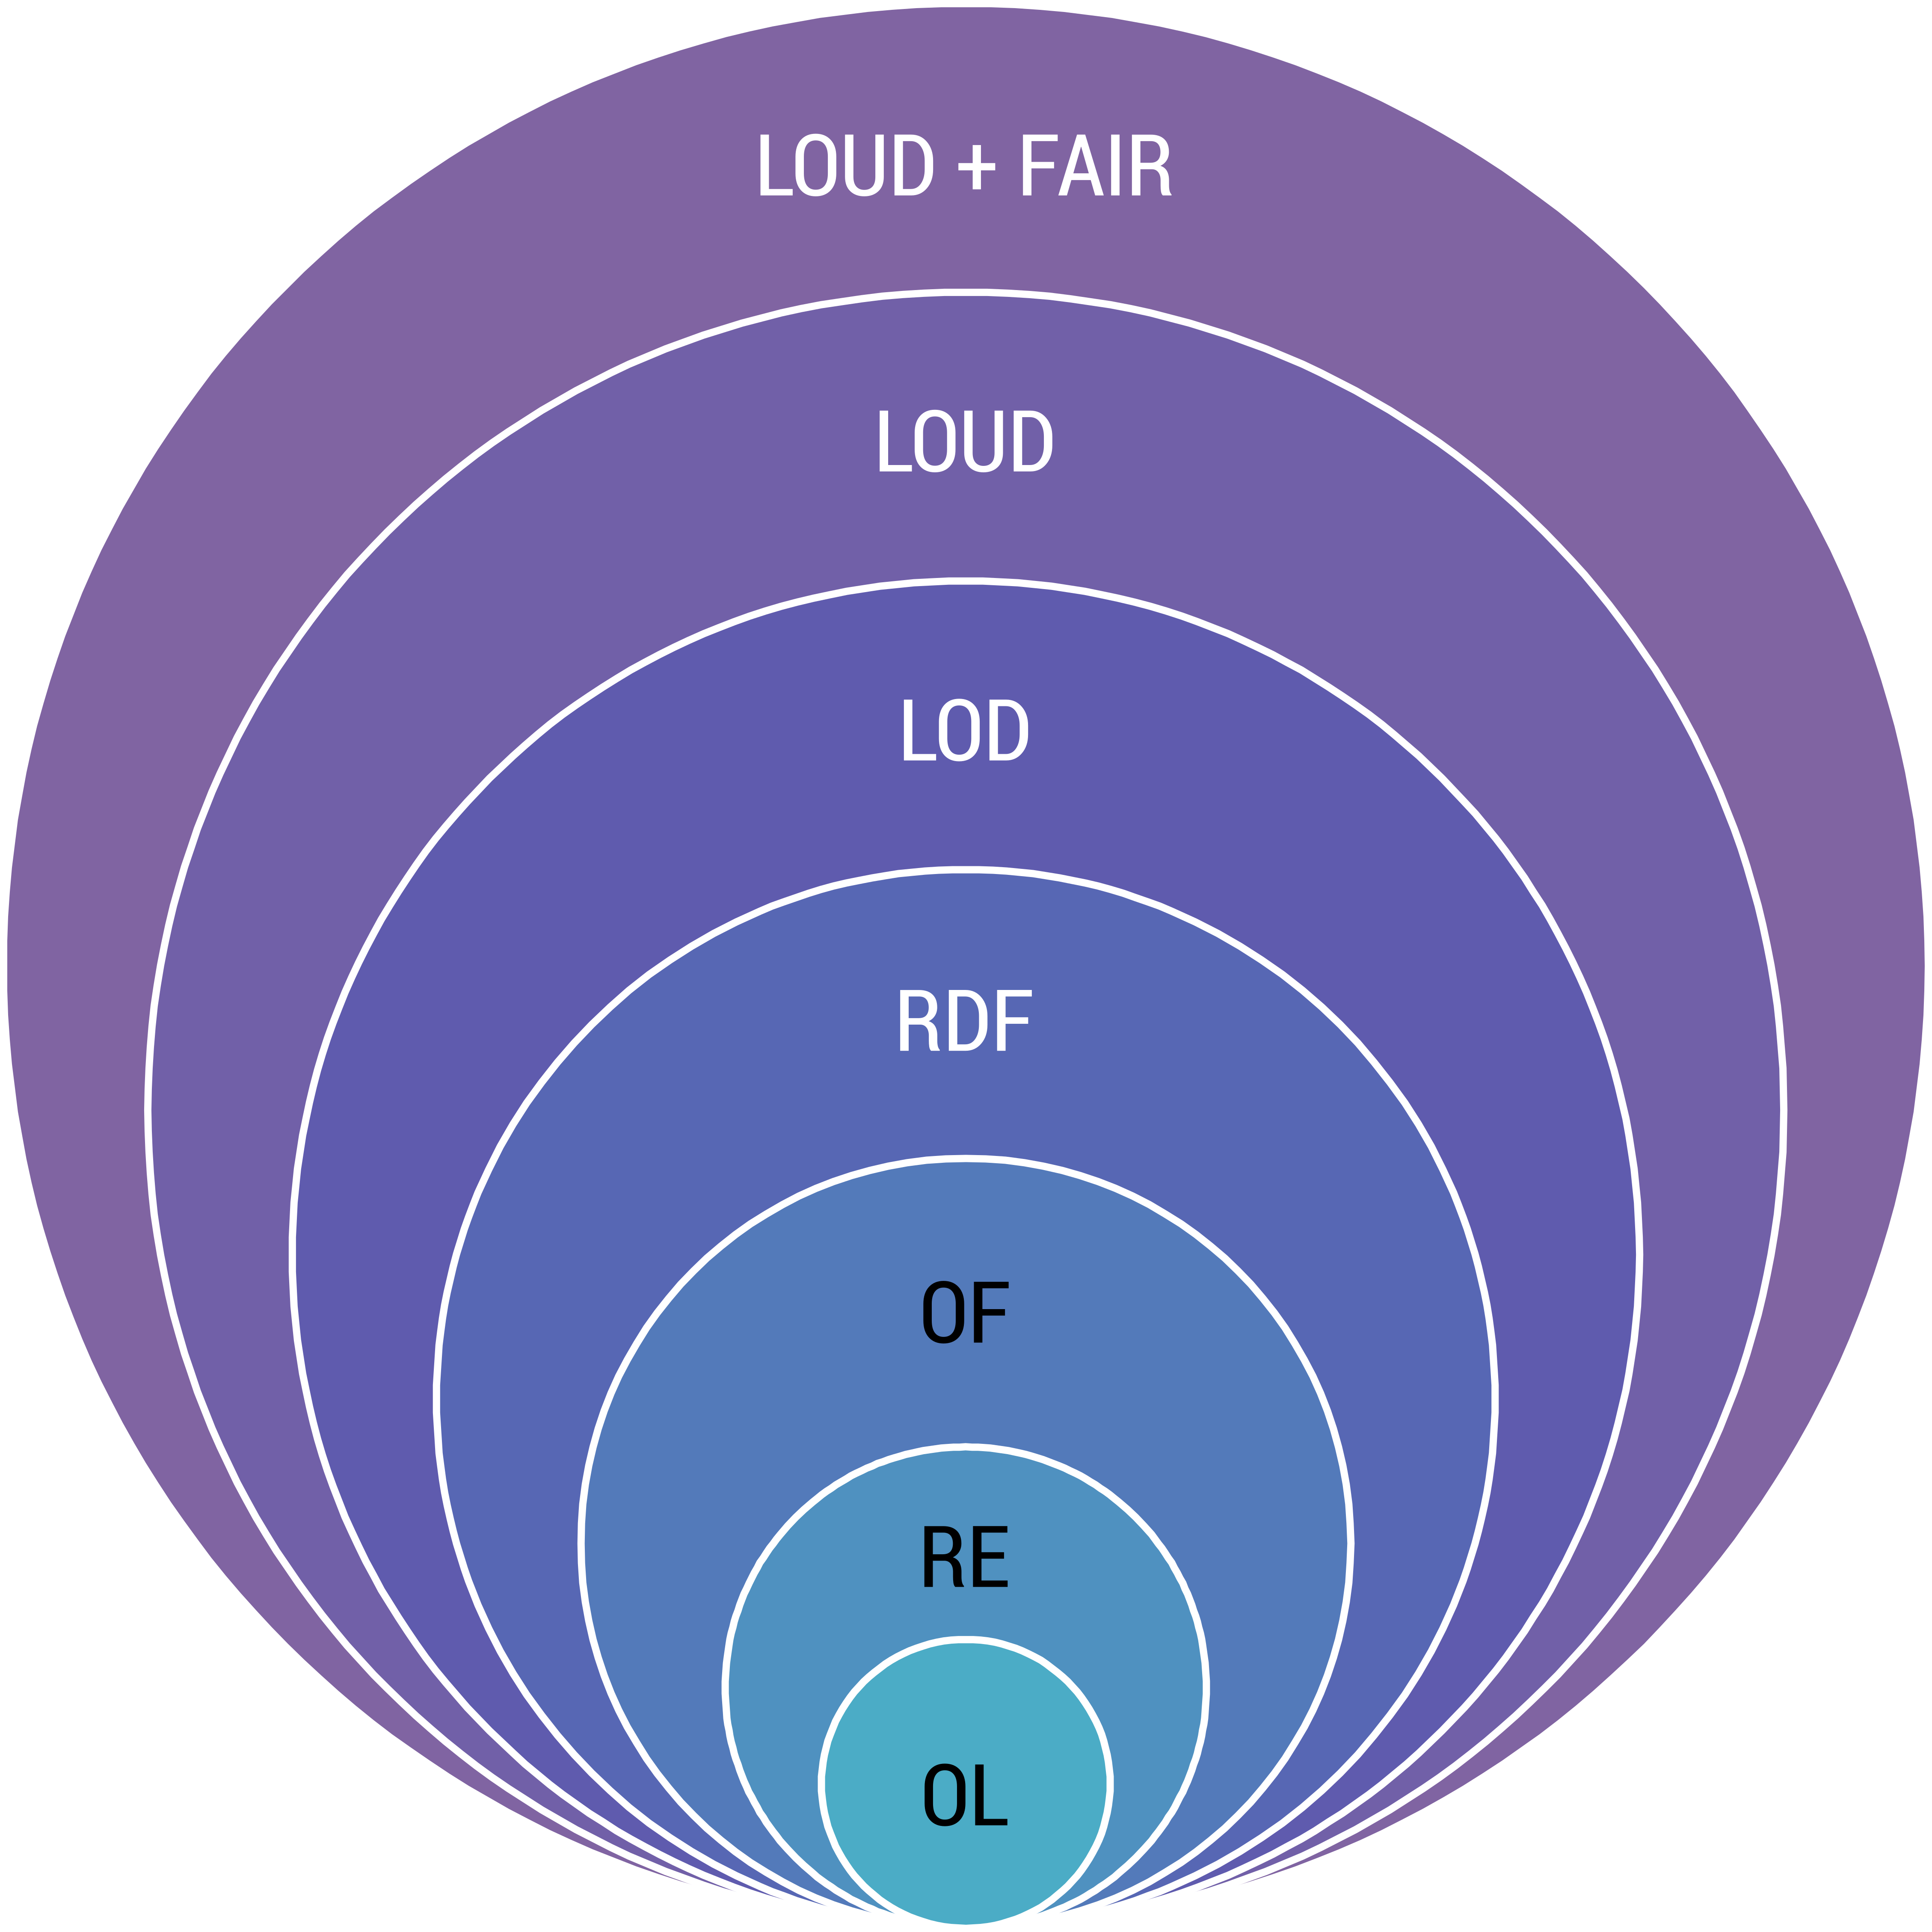
\includegraphics[width=8cm]{Loud_fair_sphere.png}
\caption{Seven Sphere Data, Florian Thiery [CC BY 4.0]}
\label{ssd}
\end{center}
\end{figure}

The \textit{Linked Data Cloud} already offers research data repositories for certain archaeological and humanities domains. Popular examples of FAIR LOUD providers are: Nomisma.org \cite{gruber_linked_2018}, Kerameikos.org \cite{gruber_linked_2015}, Pelagios \cite{isaksen_pelagios_2014}, OpenContext \cite{kansa_publishing_2007}, Portable Antiquities Scheme \cite{harper_toys_2018}, ARIADNE \cite{consiglio_nazionale_delle_ricerche_isti_enabling_2017} and there are more to come, e.g. NAVIS \cite{thiery_taming_2018_1}, ARS3D \cite{thiery_ars3d_2019} and ARIADNEplus \cite{ariadneplus_ariadneplus_2019}. 

The development of more and more repositories poses challenges in handling the complex facets of data quality and completeness. This is especially valid for archaeological data, which are based on a complicated network of concepts from different knowledge domains. Moreover, it is necessary to include means of conveying knowledge about uncertainty in the data models to produce and publish transparent FAIR and LOUD data that can also describe specific stratigraphies or the (archaeological) context of objects. In order to be able to connect different data resources, exchange standards also have to be developed, published and applied.

To enable non-experts in engaging with FAIR and especially LOUD data, small tools - \textit{minions} - were created for different purposes, such as modelling a relative chronology (Alligator \cite{seidensticker_rdf_2018}), modelling and reasoning on vague edges in graph data (Academic Meta Tool \cite{thiery_taming_2018}), creating annotated texts and images (Recogito \cite{simon_linked_2017}), and creating controlled vocabularies (Labeling System \cite{thiery_labeling_2016}). Furthermore, Wikidata \cite{mika_introducing_2014} not only offers community-driven data, but also provides a vast set of tools for using and interacting with it.

\section{Digital Dragons at CAA}

The goal of the CAA SIG on \textbf{Semantics and LOUD in Archaeology} is to bring together experts on LOD and FAIR data, as well as anybody interested in learning about FAIR and LOUD data-driven publishing, applications and research projects based on this kind of data. We would like to discuss ideas for FAIR and LOUD data models as a basis for reproducible research and exchange in the Semantic Web. The core aim of this SIG is to use the CAA’s SIG format to raise awareness for Linked Data in archaeology by creating a friendly and open platform to discuss the role of LOUD and FAIR Data in archaeology, and to enable the CAA community to learn about LOD basics. If you wish to join the SIG, feel free to contact us to be an active part of the discussion \cite{thiery_caa_2019} and help us to navigate archaeology away from the data dragons.

\bibliographystyle{IEEEtran}
\bibliography{autosam}

\end{document}